\documentclass[10pt,aspectratio=169,t]{beamer}
% \usepackage[ruled,vlined]{algorithm2e}
\usepackage{setspace}
\usepackage{hyphenat}
\usepackage{lipsum}
\usepackage{multicol}
% \usepackage[utf8]{inputenc}
\usepackage{txfonts}
\usepackage{graphicx}
\usepackage{ragged2e}
\usepackage{multirow}
\usepackage{pifont}
\usepackage[utf8]{inputenc}
\usepackage[demo]{graphicx}
\usepackage{subfig}
\setbeamertemplate{bibliography item}
{\insertbiblabel}
%
% \usetheme{AnnArbor}
% \usetheme{Hannover}


% \usetheme{Singapore}
% \usetheme{CambridgeUS}
% \usecolortheme{beaver}

% \usepackage{ragged2e}\justifying
% \setbeamertemplate{bibliography item}{~$\bullet$}%$\sbullet$
\setlength{\parskip}{5pt}
%\usepackage[style=verbose,backend=biber]{biblatex}
% \usepackage[backend=biber,style=numeric-comp,sorting=none]{biblatex}

\apptocmd{\frame}{}{\justifying}{}
%\addbibresource{paper_bib.bib}
\setbeamersize{text margin left=10mm, text margin right=10mm}
\setbeamertemplate{caption}[numbered]
\setbeamertemplate{frametitle continuation}[from second][(contd.)]
% \setbeamertemplate{frametitle continuation}{}
% [default][left, leftskip=5mm]
\setbeamerfont{footnote}{size=\tiny}
\usepackage{changepage}
% \usepackage{enumitem}
\usepackage[en-US]{datetime2}
% \renewcommand\bibliographytypesize{\small}
\usefonttheme{structuresmallcapsserif}
\usetheme{Madrid}
%\setbeamertemplate{blocks}[rounded][shadow=false]
\setbeamercolor{block body}{bg=lightgray}

\makeatletter
\renewcommand\@makefnmark{\hbox{\@textsuperscript{\usebeamercolor[fg]{footnote mark}\usebeamerfont*{footnote mark}[\@thefnmark]}}}
\renewcommand\@makefntext[1]{\@textsuperscript{\usebeamercolor[fg]{footnote mark}\usebeamerfont*{footnote mark}[\@thefnmark]}\enspace\usebeamerfont*{footnote} #1}
\makeatother
\renewcommand*{\bibfont}{\small}
%\AtBeginSection[]{
%  \begin{frame}
%    \frametitle{Table of Contents}
%    \tableofcontents[currentsection]
%  \end{frame}
%}

%----------------------------------------------------------------------
%Information to be included in the title page:
\title[Improved Foggy Object Detection]{\LARGE Vehicle Detection in Foggy Conditions}

\author[]{{
\includegraphics[height=2cm]{nitlogo.png}\\[-0.5cm]\large \\Rahul Banavathu (2006028) \\Modem Veda Sree (2006032) \\Bollina Kavya Sri(2006085)}\\[0.15cm]B.Tech(CSE)-$\langle$Semester 7$\rangle$\\ \hspace{0.35cm} \\ Under the supervision of\\Dr. Suddhasil De\\ \\}
%\author{{\large Student Name (Roll No.)}\\M.Tech.(CSE-CN)\\ \hspace{0.2cm} \\Under the supervision of\\Dr. Suddhasil De\\ [.3cm] 
\includegraphics[height=1.8cm]{nitlogo.png}}
\institute[CSE Dept., NIT Patna]{Department of Computer Science and Engineering\\National Institute of Technology Patna\\[-0.4cm]}
\DTMlangsetup{showdayofmonth=false}
\date[]{\scriptsize ~\today\\[-0.5cm]}
%\date[\tiny\today]{\scriptsize\today}

%%Information to be included in the title page:
%\title[\tiny Edge-Centric Module Placement Algorithm]{Edge-Centric Application Module Placement in Fog-Cloud}
%\author[\tiny Saurabh Kumar]{{\large Saurabh Kumar(1942005)}\\  Mtech(CSE-CN)\\ \hspace{0.2cm} \\ Under the supervision of\\Dr. Suddhasil De\\ [.3cm] 
\includegraphics[height=1.8cm]{nitlogo.png}}
%\institute[NIT Patna]{Department of CSE\\NIT Patna}
%\date[\tiny\today]{\scriptsize\today}
%% \logo{
\includegraphics[height=1cm]{nitlogo.png}}

%----------------------------------------------------------------------
\begin{document}

%--------------
\begin{frame}[plain,noframenumbering]
\maketitle
\end{frame}

%--------------
\begin{frame}
\frametitle{Outline}
\tableofcontents
\end{frame}

\newpage

%--------------
\section{Introduction}
\begin{frame}[allowframebreaks]{Introduction}

\begin{columns}
\begin{column}{1\textwidth}
\vspace{-0.5cm}
\begin{itemize}
 \justifying
\item Self-driving vehicles are going revolutionary in the field of computer science as well as automobile science.

\item But it becomes a significant challenge when the weather conditions are not ideal, e.g., foggy conditions. Which requires technological advancement in order to function accordingly.
\item Despite the availability of several robust solutions online, it becomes quite an issue in terms of accuracy while being constrained over speed. 
\item The idea of this project is to develop a solution that tackles the above mentioned problems using state-of-the-art methods available online. Of which, the one we opted is, Faster-RCNN architecture powered with the PyTorch Framework that is being trained with a dataset that contains adverse possibilites to train the model in such a way to tackle a wide range of issues.
\item Our current objective is to improve the accuracy with the least possible computational complexity.
\end{itemize}
\end{column}
\end{columns}
\end{frame}

%--------------
\section{Literature review}
\begin{frame}[allowframebreaks]{Literature review}
\vspace{-0.25cm}
\begin{block}{Summary of Related Works}
\end{block}
\vspace{-1.25cm}
\begin{columns}
\begin{column}{1\textwidth}
\vspace{0.25cm}
\begin{columns}
\begin{column}{1\textwidth}
\begin{itemize}
    \item R-CNN \cite{n4} (Region based Convolutional Neural Network)
    \begin{itemize}
        \item R-CNN uses an external region proposal algorithm to generate region proposals.
        \item It consists of an external backbone for feature extraction and an object detection head.
        \item The extracted features are then fed into a classifier to determine the presence of objects in each region.
    \end{itemize}
    \item Domain Adaptation \cite{n2}
    \begin{itemize}
        \item Labeled data from the target domain is being collected which is similar to the real world data.
        \item The backbone of the faster R-CNN will be trained on the target domain data to adapt to specific features and patterns.
        \item On the other hand, the Region Proposal Network (RPN) generates regions that are crucial to the target domain, making it more accurate.
    \end{itemize}
    
\end{itemize}
\end{column}
\end{columns}
\vspace{-0.25cm}
\end{column}
\end{columns}







\end{frame}
%--------------

\newpage


%--------------
\section{Motivation}
\begin{frame}{Motivation}
\begin{columns}
\begin{column}{1\textwidth}
\begin{itemize}
 \justifying
 \item Need of accuracy despite speed constraints.
 (from Table~\ref{Table 1}):
 \begin{itemize}
 \item Accuracy
 \begin{itemize}
  \item Accuracy of this model will be significantly promising and the speed can be improvised.
 \end{itemize}
 \item Two-staged detection
\begin{itemize}
  \item The concept of domain adaptation focuses the model towards the detection requirement. 
  \item The domain specific regions are crucially treated, which discards the unwanted regions and saves time.
 \end{itemize}
\end{itemize}

\end{itemize}
\end{column}
\end{columns}
\end{frame}
%--------------

\newpage

%--------------
\section{Problem Statement}
\begin{frame}{Problem Statement}
\begin{columns}
\begin{column}{1\textwidth}
\begin{itemize}
 \item Vehicle Detection under foggy conditions.
 \item The underlying system environment characteristics include:
 \begin{itemize}
    \item Reduced visibility in foggy images.
    \item Complex atmospheric conditions caused by haze, fog, and smoke
    \item Variability in the density of fog.
 \end{itemize}
 \item In order to:
 \begin{itemize}
  \item Surpass other Faster R-CNN models in terms of accuracy.
  \item Reduction in the running time of foggy image detection algorithms for real-time applications.
  \item To prioritize accuracy over speed.
 \end{itemize}
\end{itemize}
\end{column}
\end{columns}
\end{frame}
%--------------
\newpage
%--------------


%--------------
\section{Proposed Model}
\begin{frame}[allowframebreaks]{Proposed Model}

\vspace{-0.25cm}
\begin{block}{System Model}
\end{block}
\begin{columns}
\begin{column}{1\textwidth}
\vspace{-0.5cm}
\begin{itemize}
 \justifying
 \item Our model is an vehicle-detection system that can detect multiple and different kinds of vehicles under foggy weather conditions that are present in an image or a video.
 \item The model features two-stage domain specific detection which fine tunes the detection and predicts class probabilities for each kind of object.
 \item This model can be trained with specific foggy datasets, that consists of images with annotations that are captured in various adverse foggy conditions which enables the model to determine specific features that are posed by foggy environments.
 \item In our evaluation of the model as dual-stage object detection model, we concentrate on the accuracy and various classes of objects detected by the model.

\end{itemize}
\end{column}
\end{columns}



\end{frame}
%--------------
\newpage
\section{Architecture of Our Model}
\begin{frame}[allowframebreaks]{Architecture of Our Model}
\vspace{-0.25cm}
\begin{block}
    {Pictorial Representation}
\end{block}
\begin{columns}
\begin{column}{1\textwidth}
\begin{center}
{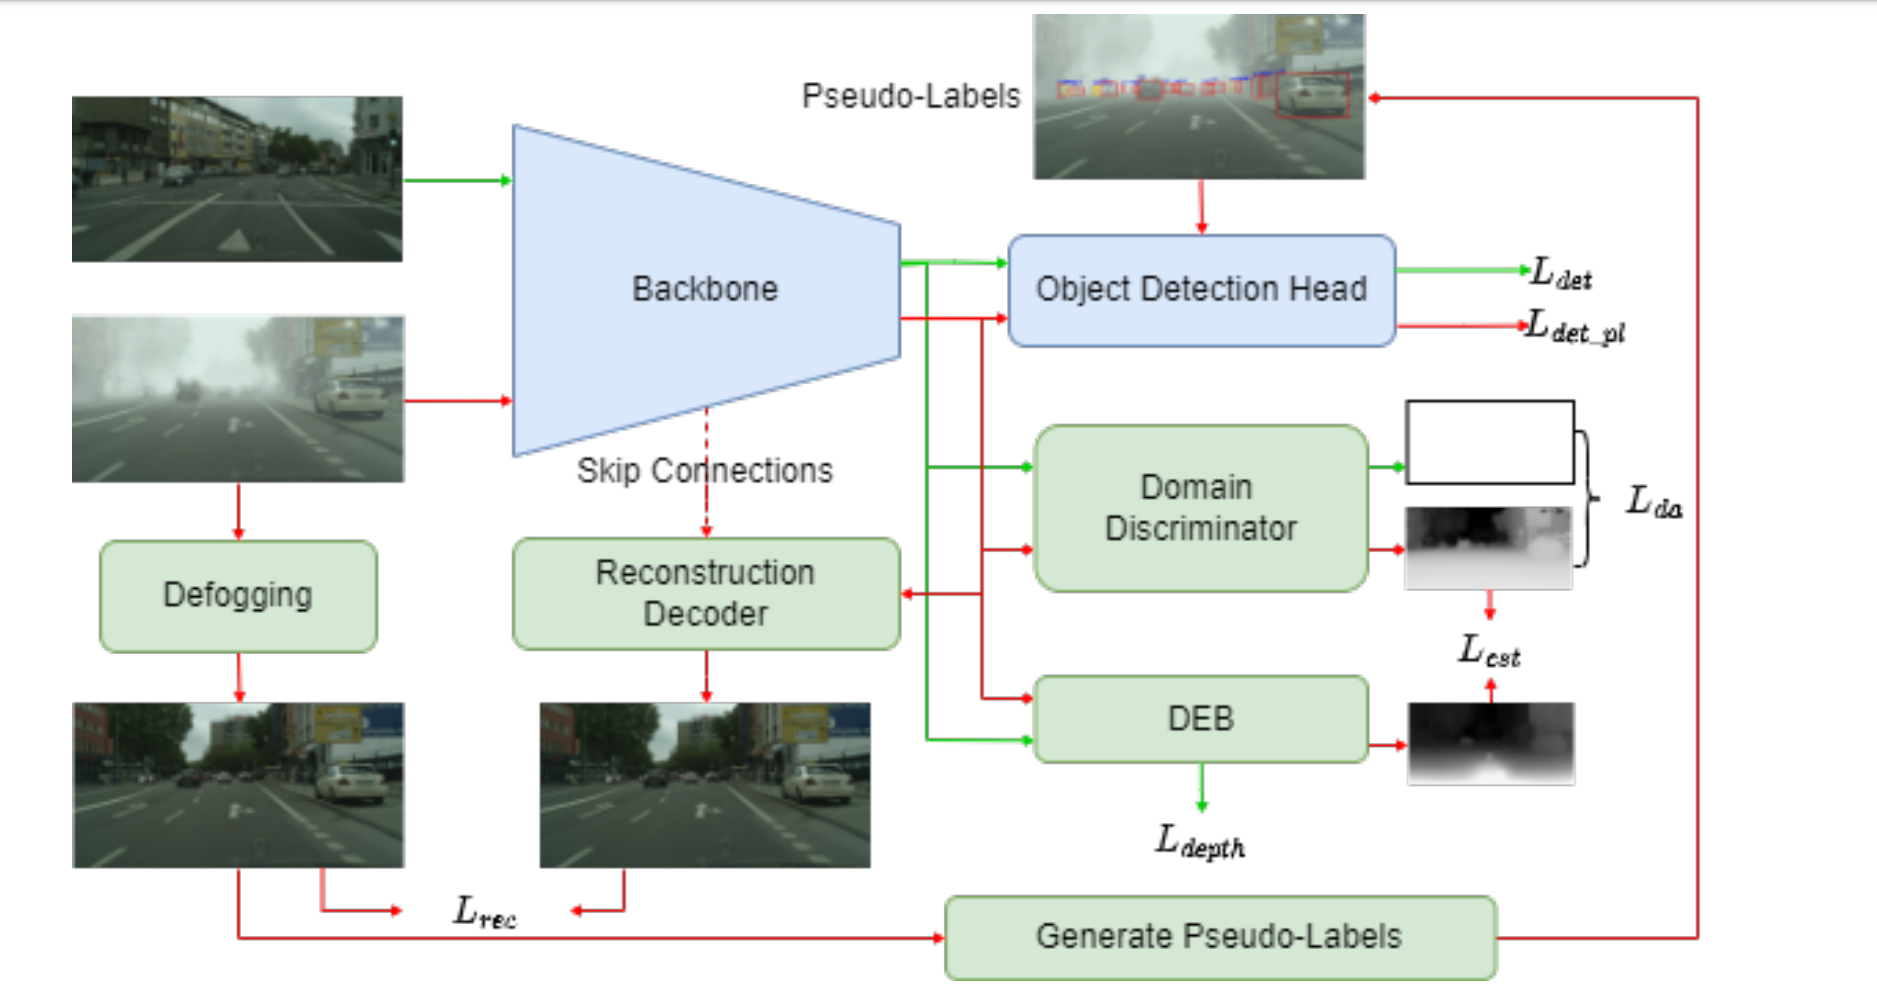
\includegraphics[height=5.5cm]{architecture.png}}
\end{center}
\end{column}
\end{columns}
\newpage
\vspace{-0.25cm}
\begin{block}
    {System Model}
\end{block}
\vspace{-0.25cm}
\begin{columns}
\begin{column}{1\textwidth}
\begin{itemize}
 \justifying
 \item The architecture of this model is convolutional neural network based that consists of two major components:
 \begin{itemize}
  \item Backbone Network
  \item Head Network
\end{itemize}
\item Backbone extracts feature maps from the input images. 
\item Object detection head localizes and categorizes object instances from the feature maps.
 \item Domain discriminator and Depth Estimation Block (DEB) encourage the backbone to extract fog-invariant features, and maintains depth distributions.
\item Reconstruction decoder minimizes the fake object features generated by Domain Adaptation (DA). 
\item Pseudo-Labels involve target domain information in the pipeline, and apply consistency regularization between fog and defogged images.
\end{itemize}
\end{column}
\end{columns}

\newpage

\begin{block}{Why this model is better than other models?}
\end{block}
\begin{columns}
\begin{column}{1\textwidth}
\vspace{-0.5cm}
\begin{itemize}
\justifying
\item  Our model is trained with a vast range of input data, which contributes to significant learning and more accurate detection.
\item A two-stage detection model along with domain adaptation improves the detection accuracy significantly with the cost of some extra time.
\item So, this model is majorly concentrated towards accuracy which includes different kinds of vehicles and detection of people too.
\item Training under various conditions and adverse scenarios ensures the enhancement of accuracy of the generated results.
\end{itemize}
\end{column}
\end{columns}


\newpage
\begin{block}{Theoritical Comparison with related works}
\end{block}
\begin{columns}
\begin{column}{1\textwidth}
\vspace{-0.5cm}
\begin{table}
\caption{Characteristics Comparison of Related works}\label{Table 1}
\centering
\begin{tabular}{ 
|p{2cm}|p{2.6cm}|p{1.9cm}|p{1cm}|p{2.3cm}|p{2.3cm}| }
 \hline
 \textbf{Reference} & \textbf{Method} & \textbf{Number of Stages} & \textbf{DeFog} & \textbf{Image Quality Reduction}  \\
 \hline
Yang X (2022) \cite{n2} & Faster R-CNN + DA  & Two Stage & YES & NO \\ \hline
Farhodov (2019) \cite{n4} & OpenCV + Faster R-CNN & Two Stage & YES & YES \\ \hline
Chin (2018) \cite{n5} & Faster R-CNN & Two Stage & NO & NO \\ \hline
\end{tabular}
\end{table}
\end{column}
\end{columns}



\end{frame}
%--------------

\section{Experimentation}
\begin{frame}[allowframebreaks]{Experimentation}

\vspace{-0.25cm}
\begin{block}{Simulation/Tentative TestBed Environment}
\end{block}
\begin{columns}
\begin{column}{1\textwidth}
\vspace{-0.5cm}
\begin{itemize}
\justifying
\item Experiment: Vehicle detection under foggy conditions. 
\item Description: This experiment involves training and testing our algorithm for vehicle detection under foggy weather conditions.
\item Hardware:
\begin{itemize}
    \item CPU: AMD Ryzen 5 4600H - 6C/12T base 3GHz and max. 4GHz with 8MB L3 Cache.
    \item Memory: Intel Optane 24GB @3200MHz CL29
    \item GPU: NVIDIA GeForce GTX1650Ti 1024C with base @1035MHz and max @1200MHz and 4GB GDDR5X VRAM.
\end{itemize}
\item Software:
\begin{itemize}
    \item OS:x64 based Windows 10 Home version 22H2 - build 19045.3448
    \item Programming Language: Python v3.10
    \item Framework: PyTorch v2.0.1 with CUDA v10.0.130 - build 411.31
\end{itemize}
\item Weather Condition: Foggy
\end{itemize}
\end{column}
\end{columns}

\newpage
\begin{block}{Experiment parameters of Our Work}
\end{block}
\begin{columns}
\begin{column}{1\textwidth}
\vspace{-0.66cm}
\begin{table}
\caption{Experiment Parameters of Our Work}\label{Table 3}
\centering
\begin{tabular}{ 
|p{5cm}|p{5cm}| }
 \hline
 \textbf{Experiment Parameters} & \textbf{Value} \\
 \hline
 Dataset & Fog Dataset with various vehicles\\
 \hline
Train, Valid, Test Data Size & 80\%, 10\%, 10\% of dataset\\
\hline
Training Framework & PyTorch\\  
\hline
Batch Size & 10\\
\hline
Epochs & 10\\
\hline 
Number of Classes &	6\\ \hline
\end{tabular}
\end{table}


\vspace{-0.65cm}
\begin{table}
\caption{Performance Metrics of Our Work}\label{Table 4}
\centering
\begin{tabular}{ 
|p{5cm}|p{7cm}| }
 \hline
 \textbf{Performance Metrics} & \textbf{Formula} \\
 \hline
 Average Precision & (TP)/(TP+FP)\\ \hline
Mean Average Precision(mAP) & Mean of Average Precision of all classes\\ \hline
\end{tabular}
\end{table}
\end{column}
\end{columns}



% \newpage
% \begin{block}{Comparison of Our Work with Related Works}
% \end{block}
% \begin{columns}
% \begin{column}{1\textwidth}
% % \vspace{-0.1cm}
% \begin{table}
% \caption{Characteristics Comparison of Our Work with Related Works}\label{Table 5}
% \centering
% % \vspace{-0cm}
% \begin{tabular}{ 
% |p{2cm}|p{1.3cm}|p{1.9cm}|p{1cm}|p{2.3cm}|p{2.3cm}| }
%  \hline
%  \textbf{Reference} & \textbf{Method} & \textbf{Number of Stages} & \textbf{DeFog} & \textbf{Image Quality Reduction} & \textbf{Instance Segmentation} \\
%  \hline

% Sun (2022)\cite{n1} & Mask R-CNN  & Two Stage & YES & YES & YES \\ \hline
% Sun (2022)\cite{n1} & SOLOv2  & Two Stage & NO & NO & YES\\ \hline
% Chin (2018)\cite{n2} & Faster R-CNN & Two Stage & NO & NO & NO\\ \hline
% Proposed Model & YOLOv5 & One Stage & NO & NO & NO\\ \hline
% \end{tabular}
% \end{table}
% \end{column}
% \end{columns}

% \newpage
% \begin{block}{Comparison of Our Work with Related Works}
% \end{block}
% \begin{columns}
% \begin{column}{1\textwidth}
% % \vspace{0.5cm}
% \begin{table}
% \caption{Performance Metrics Comparison of our work with Related Works}\label{Table 6}
% \centering
% \begin{tabular}{ 
% |p{2cm}|p{1cm}|p{1.2cm}|p{1.2cm}|p{1cm}|p{1cm}|p{1cm}|p{1cm}| }
%  \hline
%  \textbf{Reference} & \textbf{mAP} & \textbf{mAP50} & \textbf{mAP75} & \textbf{mAPs} & \textbf{mAPm} & \textbf{mAPl}  \\ \hline
% Sun (2022)\cite{n1} & 39.41 & 73.95 &  38.07 & 20.38 & 43.41 & 47.18 \\ \hline
% Sun (2022)\cite{n1} & 44.51  & 76.2 & 43.5 & 14.79 & 40.41 & 63.96\\ \hline
% Chin (2018)\cite{n2} & 34.90 & 55.70 & 37.40 & 15.60 & 38.70 & 50.90\\ \hline
% Proposed Model & 78.20 & 76.30 & 52.10 & 27.30 & 51.50 & 64.20\\ \hline
 
% \end{tabular}
% \end{table}
% \end{column}
% \end{columns}



\end{frame}

% %--------------

\section{Works To Be Done}
\begin{frame}{Works To Be Done}
\begin{columns}
\begin{column}{1\textwidth}
\begin{itemize}
\justifying
\item To train the model with a proper annotated dataset for 1st iteration.
\item To expand the train dataset in an iterative manner.
\item To maintain or to increase the accuracy with increased dataset size.
\item To expand the objects classification by empowering domain adaptation with depth-embedding for specific feature extraction.
\end{itemize}
\end{column}
\end{columns}
\end{frame}


%--------------

\section{References}
\begin{frame}[allowframebreaks] {References}
\begin{thebibliography}{9}
  \bibitem{n1} Li, Chengyang, et al. "Detection-friendly dehazing: Object detection in real-world hazy scenes." IEEE Transactions on Pattern Analysis and Machine Intelligence (2023).
\bibitem{n2}Yang, X., Mi, M. B., Yuan, Y., Wang, X., & Tan, R. T. (2022). Object Detection in Foggy Scenes by Embedding Depth and Reconstruction into Domain Adaptation. In Proceedings of the Asian Conference on Computer Vision (pp. 1093-1108).
\bibitem{n3} Sun, Yuxin, et al. "Global Mask R-CNN for marine ship instance segmentation." Neurocomputing 480 (2022): 257-270.
\bibitem{n4} Farhodov, X., Kwon, O. H., Kang, K. W., Lee, S. H., & Kwon, K. R. (2019, November). Faster RCNN detection based OpenCV CSRT tracker using drone data. In 2019 International Conference on Information Science and Communications Technologies (ICISCT) (pp. 1-3). IEEE.
 \bibitem{n5} Chen, Y., Li, W., Sakaridis, C., Dai, D., & Van Gool, L. (2018). Domain adaptive faster r-cnn for object detection in the wild. In Proceedings of the IEEE conference on computer vision and pattern recognition (pp. 3339-3348).
\bibitem{n6} Liu, Shu, Lu Qi, Haifang Qin, Jianping Shi, and Jiaya Jia. "Path aggregation network for instance segmentation." In Proceedings of the IEEE conference on computer vision and pattern recognition, pp. 8759-8768. 2018.

 \end{thebibliography}
 \end{frame}
\newpage

%--------------

\begin{frame}[plain,noframenumbering]
\vspace{3.2cm}
\begin{center}
{\fontsize{40}{50}\selectfont THANK YOU}
\end{center}
\end{frame}
%--------------


\end{document}